\documentclass[a4paper,14pt,oneside,openany]{memoir}

%%% Задаем поля, отступы и межстрочный интервал %%%

\usepackage[left=30mm, right=15mm, top=20mm, bottom=20mm]{geometry} % Пакет geometry с аргументами для определения полей
\pagestyle{plain} % Убираем стандарные для данного класса верхние колонтитулы с заголовком текущей главы, оставляем только номер страницы снизу по центру
\parindent=1.25cm % Абзацный отступ 1.25 см, приблизительно равно пяти знакам, как по ГОСТ
\usepackage{indentfirst} % Добавляем отступ к первому абзацу
%\linespread{1.3} % Межстрочный интервал (наиболее близко к вордовскому полуторному) - тут вместо этого используется команда OnehalfSpacing*

%%% Задаем языковые параметры и шрифт %%%

\usepackage[english, russian]{babel}                % Настройки для русского языка как основного в тексте
\babelfont{rm}{Times New Roman}                     % TMR в качестве базового roman-щрифта

%%% Задаем стиль заголовков и подзаголовков в тексте %%%

\setsecnumdepth{subsection} % Номера разделов считать до третьего уровня включительно, т.е. нумеруются только главы, секции, подсекции
\renewcommand*{\chapterheadstart}{} % Переопределяем команду, задающую отступ над заголовком, чтобы отступа не было
\renewcommand*{\printchaptername}{} % Переопределяем команду, печатающую слово "Глава", чтобы оно не печалось
%\renewcommand*{\printchapternum}{} % То же самое для номера главы - тут не надо, номер главы оставляем
\renewcommand*{\chapnumfont}{\normalfont\bfseries} % Меняем стиль шрифта для номера главы: нормальный размер, полужирный
\renewcommand*{\afterchapternum}{\hspace{1em}} % Меняем разделитель между номером главы и названием
\renewcommand*{\printchaptertitle}{\normalfont\bfseries\centering\MakeUppercase} % Меняем стиль написания для заголовка главы: нормальный размер, полужирный, центрированный, заглавными буквами
\setbeforesecskip{20pt} % Задаем отступ перед заголовком секции
\setaftersecskip{20pt} % Ставим такой же отступ после заголовка секции
\setsecheadstyle{\raggedright\normalfont\bfseries} % Меняем стиль написания для заголовка секции: выравнивание по правому краю без переносов, нормальный размер, полужирный
\setbeforesubsecskip{20pt} % Задаем отступ перед заголовком подсекции
\setaftersubsecskip{20pt} % Ставим такой же отступ после заголовка подсекции
\setsubsecheadstyle{\raggedright\normalfont\bfseries}  % Меняем стиль написания для заголовка подсекции: выравнивание по правому краю без переносов, нормальный размер, полужирный

%%% Задаем параметры оглавления %%%

\addto\captionsrussian{\renewcommand\contentsname{Содержание}} % Меняем слово "Оглавление" на "Содержание"
\setrmarg{2.55em plus1fil} % Запрещаем переносы слов в оглавлении
%\setlength{\cftbeforechapterskip}{0pt} % Эта команда убирает интервал между заголовками глав - тут не надо, так красивее смотрится
\renewcommand{\aftertoctitle}{\afterchaptertitle \vspace{-\cftbeforechapterskip}} % Делаем отступ между словом "Содержание" и первой строкой таким же, как у заголовков глав
%\renewcommand*{\chapternumberline}[1]{} % Делаем так, чтобы номер главы не печатался - тут не надо
\renewcommand*{\cftchapternumwidth}{1.5em} % Ставим подходящий по размеру разделитель между номером главы и самим заголовком
\renewcommand*{\cftchapterfont}{\normalfont\MakeUppercase} % Названия глав обычным шрифтом заглавными буквами
\renewcommand*{\cftchapterpagefont}{\normalfont} % Номера страниц обычным шрифтом
\renewcommand*{\cftchapterdotsep}{\cftdotsep} % Делаем точки до номера страницы после названий глав
\renewcommand*{\cftdotsep}{1} % Задаем расстояние между точками
\renewcommand*{\cftchapterleader}{\cftdotfill{\cftchapterdotsep}} % Делаем точки стандартной формы (по умолчанию они "жирные")
\maxtocdepth{subsection} % В оглавление попадают только разделы первыхтрех уровней: главы, секции и подсекции

%%% Выравнивание и переносы %%%

%% http://tex.stackexchange.com/questions/241343/what-is-the-meaning-of-fussy-sloppy-emergencystretch-tolerance-hbadness
%% http://www.latex-community.org/forum/viewtopic.php?p=70342#p70342
\tolerance 1414
\hbadness 1414
\emergencystretch 1.5em                             % В случае проблем регулировать в первую очередь
\hfuzz 0.3pt
\vfuzz \hfuzz
%\dbottom
%\sloppy                                            % Избавляемся от переполнений
\clubpenalty=10000                                  % Запрещаем разрыв страницы после первой строки абзаца
\widowpenalty=10000                                 % Запрещаем разрыв страницы после последней строки абзаца
\brokenpenalty=4991                                 % Ограничение на разрыв страницы, если строка заканчивается переносом

%%% Объясняем компилятору, какие буквы русского алфавита можно использовать в перечислениях (подрисунках и нумерованных списках) %%%
%%% По ГОСТ нельзя использовать буквы ё, з, й, о, ч, ь, ы, ъ %%%
%%% Здесь также переопределены заглавные буквы, хотя в принципе они в документе не используются %%%

\makeatletter
    \def\russian@Alph#1{\ifcase#1\or
       А\or Б\or В\or Г\or Д\or Е\or Ж\or
       И\or К\or Л\or М\or Н\or
       П\or Р\or С\or Т\or У\or Ф\or Х\or
       Ц\or Ш\or Щ\or Э\or Ю\or Я\else\xpg@ill@value{#1}{russian@Alph}\fi}
    \def\russian@alph#1{\ifcase#1\or
       а\or б\or в\or г\or д\or е\or ж\or
       и\or к\or л\or м\or н\or
       п\or р\or с\or т\or у\or ф\or х\or
       ц\or ш\or щ\or э\or ю\or я\else\xpg@ill@value{#1}{russian@alph}\fi}
\makeatother

%%% Задаем параметры оформления рисунков и таблиц %%%

\usepackage{graphicx, caption, subcaption} % Подгружаем пакеты для работы с графикой и настройки подписей
\graphicspath{{images/}} % Определяем папку с рисунками
\captionsetup[figure]{font=small, width=\textwidth, name=Рисунок, justification=centering} % Задаем параметры подписей к рисункам: маленький шрифт (в данном случае 12pt), ширина равна ширине текста, полнотекстовая надпись "Рисунок", выравнивание по центру
\captionsetup[subfigure]{font=small} % Индексы подрисунков а), б) и так далее тоже шрифтом 12pt (по умолчанию делает еще меньше)
\captionsetup[table]{singlelinecheck=false,font=small,width=\textwidth,justification=justified} % Задаем параметры подписей к таблицам: запрещаем переносы, маленький шрифт (в данном случае 12pt), ширина равна ширине текста, выравнивание по ширине
\captiondelim{ --- } % Разделителем между номером рисунка/таблицы и текстом в подписи является длинное тире
\setkeys{Gin}{width=\textwidth} % По умолчанию размер всех добавляемых рисунков будет подгоняться под ширину текста
\renewcommand{\thesubfigure}{\asbuk{subfigure}} % Нумерация подрисунков строчными буквами кириллицы
%\setlength{\abovecaptionskip}{0pt} % Отбивка над подписью - тут не меняем
%\setlength{\belowcaptionskip}{0pt} % Отбивка под подписью - тут не меняем
\usepackage[section]{placeins} % Объекты типа float (рисунки/таблицы) не вылезают за границы секциии, в которой они объявлены

%%% Задаем параметры ссылок и гиперссылок %%% 

\usepackage{hyperref}                               % Подгружаем нужный пакет
\hypersetup{
    colorlinks=true,                                % Все ссылки и гиперссылки цветные
    linktoc=all,                                    % В оглавлении ссылки подключатся для всех отображаемых уровней
    linktocpage=true,                               % Ссылка - только номер страницы, а не весь заголовок (так выглядит аккуратнее)
    linkcolor=red,                                  % Цвет ссылок и гиперссылок - красный
    citecolor=red                                   % Цвет цитировний - красный
}

%%% Настраиваем отображение списков %%%

\usepackage{enumitem}                               % Подгружаем пакет для гибкой настройки списков
\renewcommand*{\labelitemi}{\normalfont{--}}        % В ненумерованных списках для пунктов используем короткое тире
\makeatletter
    \AddEnumerateCounter{\asbuk}{\russian@alph}     % Объясняем пакету enumitem, как использовать asbuk
\makeatother
\renewcommand{\labelenumii}{\asbuk{enumii})}        % Кириллица для второго уровня нумерации
\renewcommand{\labelenumiii}{\arabic{enumiii})}     % Арабские цифры для третьего уровня нумерации
\setlist{noitemsep, leftmargin=*}                   % Убираем интервалы между пунками одного уровня в списке
\setlist[1]{labelindent=\parindent}                 % Отступ у пунктов списка равен абзацному отступу
\setlist[2]{leftmargin=\parindent}                  % Плюс еще один такой же отступ для следующего уровня
\setlist[3]{leftmargin=\parindent}                  % И еще один для третьего уровня

%%% Счетчики для нумерации объектов %%%

\counterwithout{figure}{chapter}                    % Сквозная нумерация рисунков по документу
\counterwithout{equation}{chapter}                  % Сквозная нумерация математических выражений по документу
\counterwithout{table}{chapter}                     % Сквозная нумерация таблиц по документу

%%% Реализация библиографии пакетами biblatex и biblatex-gost с использованием движка biber %%%

\usepackage{csquotes} % Пакет для оформления сложных блоков цитирования (biblatex рекомендует его подключать)
\usepackage[%
backend=biber,                                      % Движок
bibencoding=utf8,                                   % Кодировка bib-файла
sorting=none,                                       % Настройка сортировки списка литературы
style=gost-numeric,                                 % Стиль цитирования и библиографии по ГОСТ
language=auto,                                      % Язык для каждой библиографической записи задается отдельно
autolang=other,                                     % Поддержка многоязычной библиографии
sortcites=true,                                     % Если в квадратных скобках несколько ссылок, то отображаться будут отсортированно
movenames=false,                                    % Не перемещать имена, они всегда в начале библиографической записи
maxnames=5,                                         % Максимальное отображаемое число авторов
minnames=3,                                         % До скольки сокращать число авторов, если их больше максимума
doi=false,                                          % Не отображать ссылки на DOI
isbn=false,                                         % Не показывать ISBN, ISSN, ISRN
]{biblatex}[2016/09/17]
\DeclareDelimFormat{bibinitdelim}{}                 % Убираем пробел между инициалами (Иванов И.И. вместо Иванов И. И.)
\addbibresource{biba.bib}                           % Определяем файл с библиографией

%%% Скрипт, который автоматически подбирает язык (и, следовательно, формат) для каждой библиографической записи %%%
%%% Если в названии работы есть кириллица - меняем значение поля langid на russian %%%
%%% Все оставшиеся пустые места в поле langid заменяем на english %%%

\DeclareSourcemap{
  \maps[datatype=bibtex]{
    \map{
        \step[fieldsource=title, match=\regexp{^\P{Cyrillic}*\p{Cyrillic}.*}, final]
        \step[fieldset=langid, fieldvalue={russian}]
    }
    \map{
        \step[fieldset=langid, fieldvalue={english}]
    }
  }
}

%%% Прочие пакеты для расширения функционала %%%

\usepackage{longtable,ltcaption}                    % Длинные таблицы
\usepackage{multirow,makecell}                      % Улучшенное форматирование таблиц
\usepackage{booktabs}                               % Еще один пакет для красивых таблиц
\usepackage{soulutf8}                               % Поддержка переносоустойчивых подчёркиваний и зачёркиваний
\usepackage{icomma}                                 % Запятая в десятичных дробях
\usepackage{hyphenat}                               % Для красивых переносов
\usepackage{textcomp}                               % Поддержка "сложных" печатных символов типа значков иены, копирайта и т.д.
\usepackage[version=4]{mhchem}                      % Красивые химические уравнения
\usepackage{amsmath}                                % Усовершенствование отображения математических выражений 
\usepackage{listings}
\usepackage{xcolor}
\usepackage{graphicx}
\usepackage{epstopdf} %%package to overcome problem with eps in pdf files
\usepackage{amsmath}
\usepackage{amsfonts}

% \usepackage{amsthm}
% \usepackage{tcolorbox}
% \usepackage{floatrow}
% \usepackage{tabularx}
% % \usepackage[bottom]{footmisc} 
% \usepackage{titleps}
% \usepackage{breqn}
%%% Вставляем по очереди все содержательные части документа %%%

\begin{document}

\thispagestyle{empty}

\begin{center}
    МИНИСТЕРСТВО НАУКИ И ВЫСШЕГО ОБРАЗОВАНИЯ \\ РОССИЙСКОЙ ФЕДЕРАЦИИ

    \vspace{20pt}

    Университет ИТМО

    \vspace{20pt}

    Факультет систем управления и робототехники
\end{center}

\vfill

\begin{center}
    ОТЧЁТ \\  
    по дисциплине \\
    \textit{"Частотные методы"}

    \vspace{20pt}

    по теме: \\
    \uppercase{Жёсткая фильтрация}
\end{center}

\vfill

    \noindent Студент: \\
    \textit{Группа R3236 \hfill Поляков А.А.}

    \vspace{20pt}

    \noindent Предподаватель: \\
    \textit{к.т.н., доцент \hfill Перегудин А.А.}

\vfill

\begin{center}
    Санкт-Петербург \\ 2024
\end{center}                                     % Титульник

\newpage % Переходим на новую страницу
\setcounter{page}{2} % Начинаем считать номера страниц со второй
\OnehalfSpacing* % Задаем полуторный интервал текста (в титульнике одинарный, поэтому команда стоит после него)

\tableofcontents*                                   % Автособираемое оглавление
                            
\chapter{Задание 1. Спектральное дифференцирование}
\label{ch:chap1}

\definecolor{codegreen}{rgb}{0,0.6,0}
\definecolor{codegray}{rgb}{0.5,0.5,0.5}
\definecolor{codepurple}{rgb}{0.58,0,0.82}
\definecolor{backcolour}{rgb}{0.95,0.95,0.92}

\lstdefinestyle{mystyle}{
    backgroundcolor=\color{backcolour},   
    commentstyle=\color{codegreen},
    keywordstyle=\color{magenta},
    numberstyle=\tiny\color{codegray},
    stringstyle=\color{codepurple},
    basicstyle=\ttfamily\footnotesize,
    breakatwhitespace=false,         
    breaklines=true,                 
    captionpos=b,                    
    keepspaces=true,                 
    numbers=left,                    
    numbersep=5pt,                  
    showspaces=false,                
    showstringspaces=false,
    showtabs=false,                  
    tabsize=2
}

\lstset{style=mystyle}

\section{Лирическое вступление}

В данном задании мы рассматриваем сигнал \texttt{y=sin(t)} с небольшим шумом уже знакомого вида - \texttt{a*(rand(size(t))-0.5)}

Для начала найдём численную производную от зашумлённого сигнала через поэлементную формулу: $$\frac{y(k+1) - y(k)}{dt}$$

Найдём численную спектральную производную от зашумлённого сигнала, использую свойство Фурье-оператора: $$\mathbb{F}(\frac{df}{dt}) = 2\pi i \nu\mathbb{F}(f)$$

То есть, сначала мы получаем Фурье-образ от обычного сигнала, потом домнажаем поэлементно на константы, это нас сразу сводит в Фурье-образ производной от сигнала, а теперь возвращаемся в мир обыкновенных сигналов с помощью обратного преобразования Фурье.

\newpage
\section{Графики компонент Фурье-образа сигнала и его спектральной производной}

\begin{figure}[ht]
    \centering
    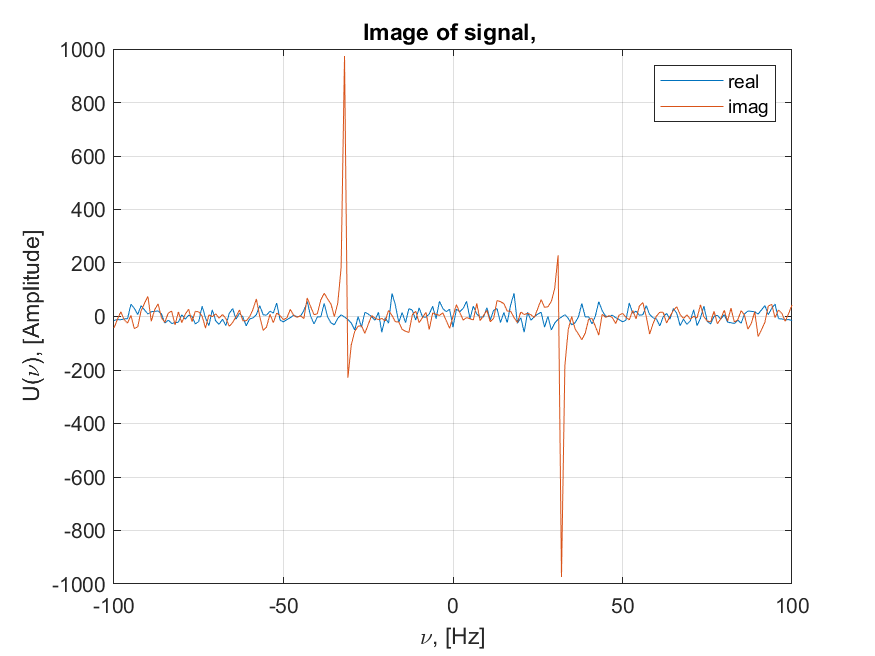
\includegraphics[width=0.7\textwidth]{image_of_numeric_diff_signal.png}
	\caption{Фурье-образ численной производной сигнала}
\end{figure}

\begin{figure}[ht]
    \centering
    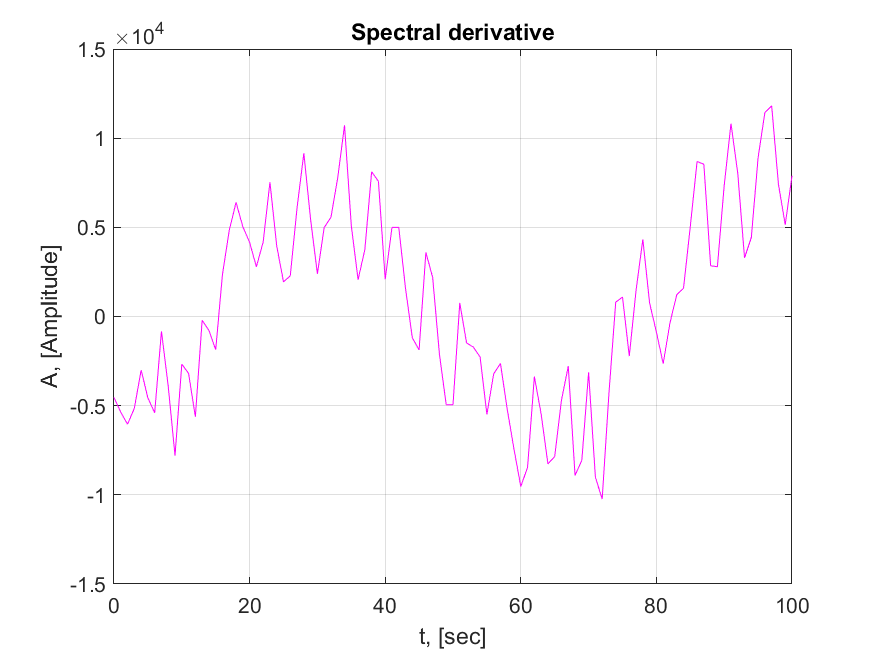
\includegraphics[width=0.7\textwidth]{spectral_diff.png}
	\caption{Спектральная производная}
\end{figure}

\newpage
\section{Графики для сравнения}

\begin{figure}[ht]
    \centering
    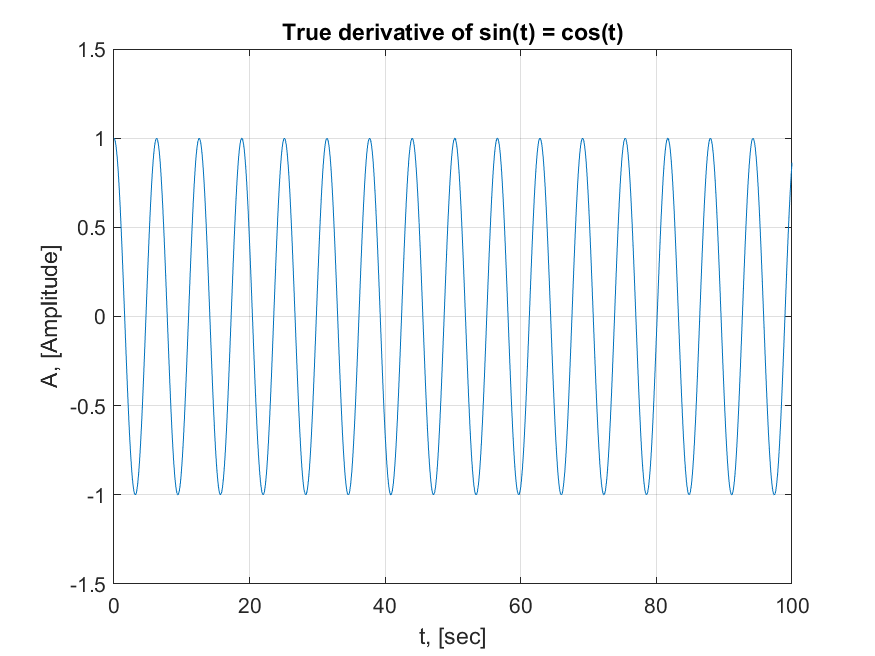
\includegraphics[width=0.7\textwidth]{true_diff.png}
	\caption{Истинная производная}
\end{figure}

\begin{figure}[ht]
    \centering
    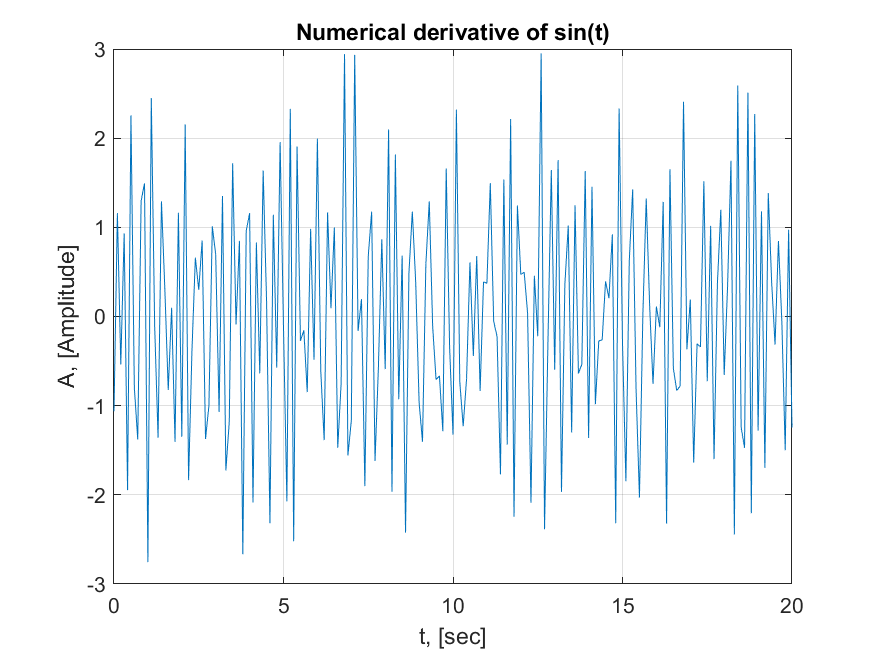
\includegraphics[width=0.5\textwidth]{numerical_diff.png}
	\caption{Численная производная}
\end{figure}

\begin{figure}[ht]
    \centering
    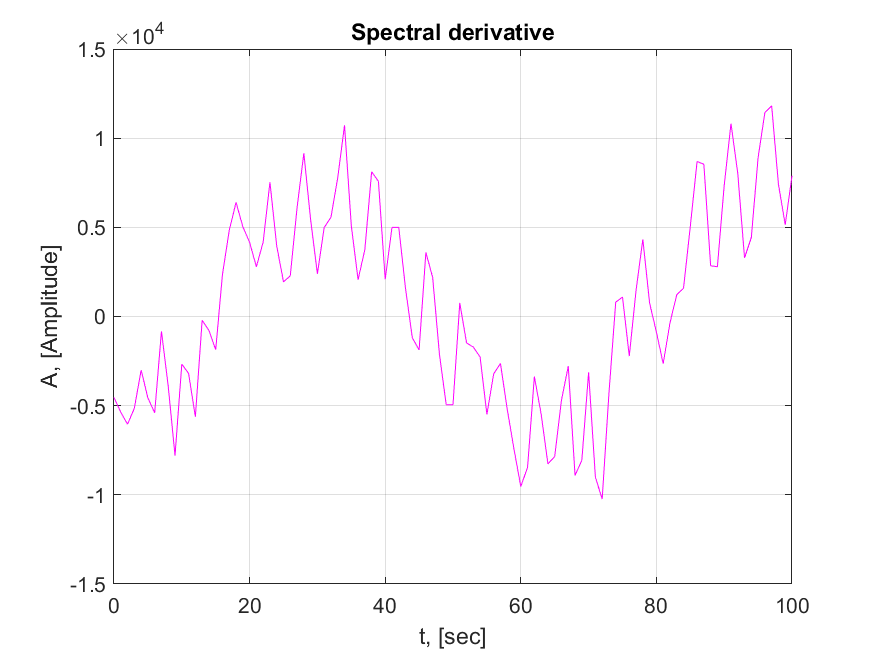
\includegraphics[width=0.7\textwidth]{spectral_diff.png}
	\caption{Спектральная производная}
\end{figure}

\newpage
\section{Делаем выводы}

Если не приближать и не рассматривать эти три графика вблизи, то кажется, что численная и спектральная - \textit{просто гармонический шум}... Если подобрать удачные отрезки рассмотрения, то прослеживается тот факт, что они очень сильно хотят напоминать график оригинальной производной, но не могут.
Думаю, что основное достижение сейчас - это то, что \textbf{мы смогли получить производную} без численного приближения только с помощью оператора Фурье и прямого, обратного преобразования.

\endinput
\chapter{Задание 1. Линейные фильтры}
\label{ch:chap2}

\definecolor{codegreen}{rgb}{0,0.6,0}
\definecolor{codegray}{rgb}{0.5,0.5,0.5}
\definecolor{codepurple}{rgb}{0.58,0,0.82}
\definecolor{backcolour}{rgb}{0.95,0.95,0.92}

\lstdefinestyle{mystyle}{
    backgroundcolor=\color{backcolour},   
    commentstyle=\color{codegreen},
    keywordstyle=\color{magenta},
    numberstyle=\tiny\color{codegray},
    stringstyle=\color{codepurple},
    basicstyle=\ttfamily\footnotesize,
    breakatwhitespace=false,         
    breaklines=true,                 
    captionpos=b,                    
    keepspaces=true,                 
    numbers=left,                    
    numbersep=5pt,                  
    showspaces=false,                
    showstringspaces=false,
    showtabs=false,                  
    tabsize=2
}
\lstset{style=mystyle}

Возьмём шумный сигнал из прошлой лабы, но будем применять оружие покрупнее:
$$
\texttt{u = g + b*(rand(size(t))-0.5) + c*sin(d*t);}
$$

\section{Фильтр первого порядка}
Линейный фильтр первого порядка мы зададим следующим образом:
$$ W_1(p)=\frac{1}{Tp + 1}$$

Берём $d=c=0$, также зададим постоянную времени $T > 0$ для фильтра. Тогда в этом пункте мы будем работать со следующей версией шумного сигнала:
$$\texttt{u = g + b*(rand(size(t))-0.5)}$$
\dots из чего сразу следует, что у нас добавляется только "случайный" шум.

\subsection{Испытания}
Построим сравнительные графики исходного и фильтрованного сигналов, графики модулей их Фурье-образов, а также АЧХ  и ФЧХ фильтра. 
Чтобы возможно упростить общий анализ, я свёл все эти графики в подграфики.


\begin{figure}[ht]
    \centering
    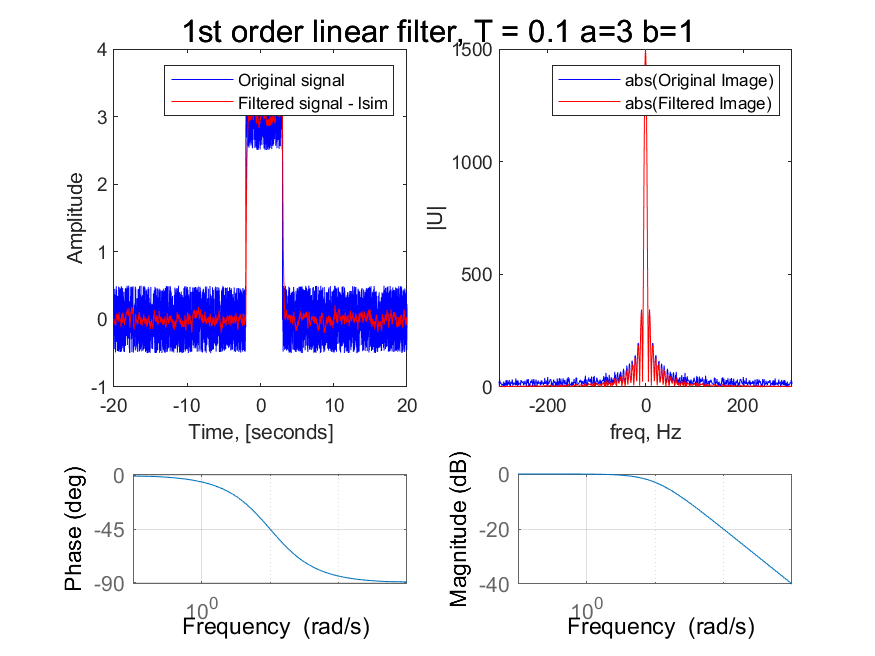
\includegraphics[width=1\textwidth]{test_linear_filter=3_b=1_T=0_10.png}
	\caption{Испытание 1}
\end{figure}

\begin{figure}[ht]
    \centering
    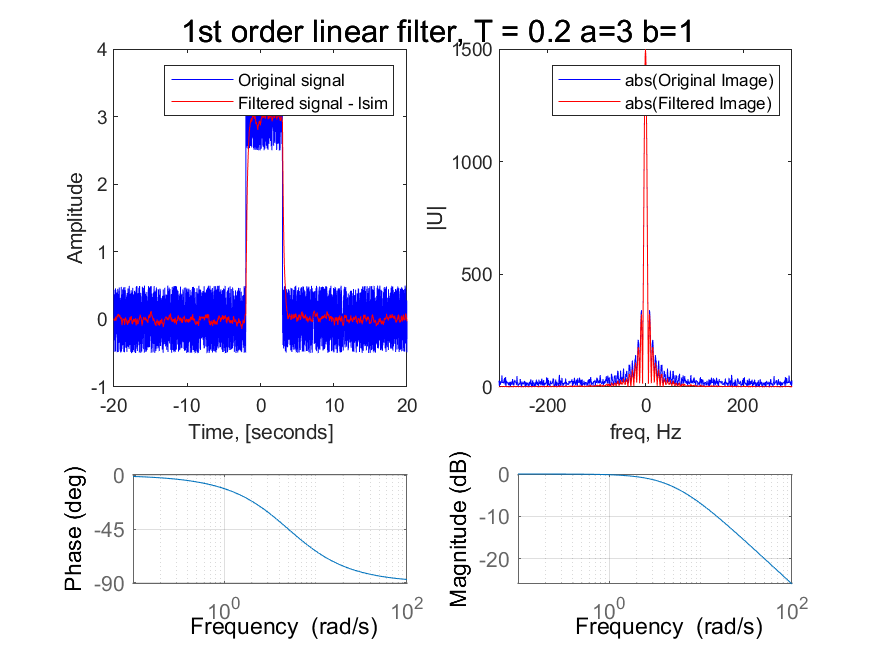
\includegraphics[width=1\textwidth]{test_linear_filter=3_b=1_T=0_20.png}
	\caption{Испытание 2}
\end{figure}

\begin{figure}[ht]
    \centering
    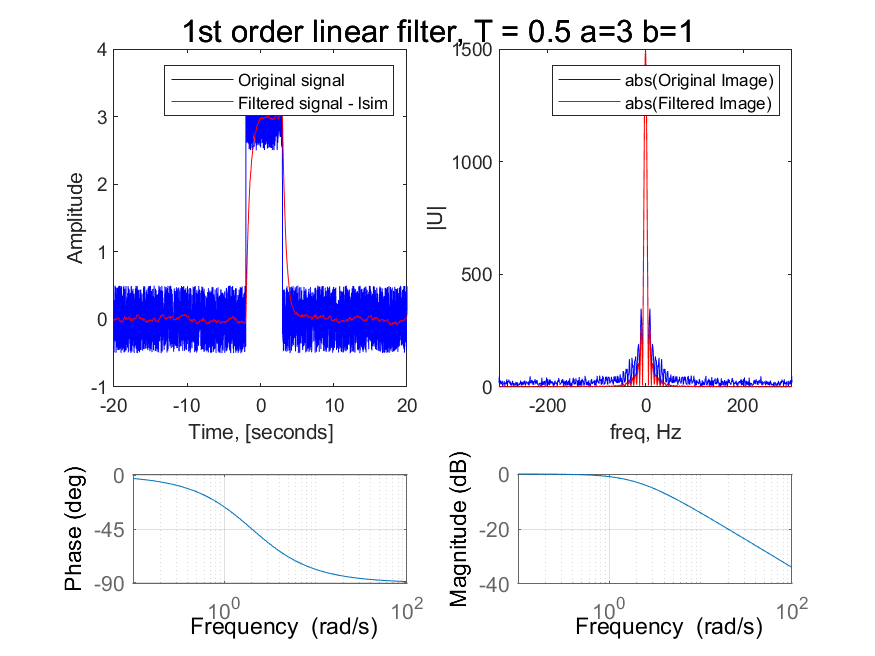
\includegraphics[width=1\textwidth]{test_linear_filter=3_b=1_T=0_50.png }
	\caption{Испытание 3}
\end{figure}
\newpage
\begin{figure}[ht]
    \centering
    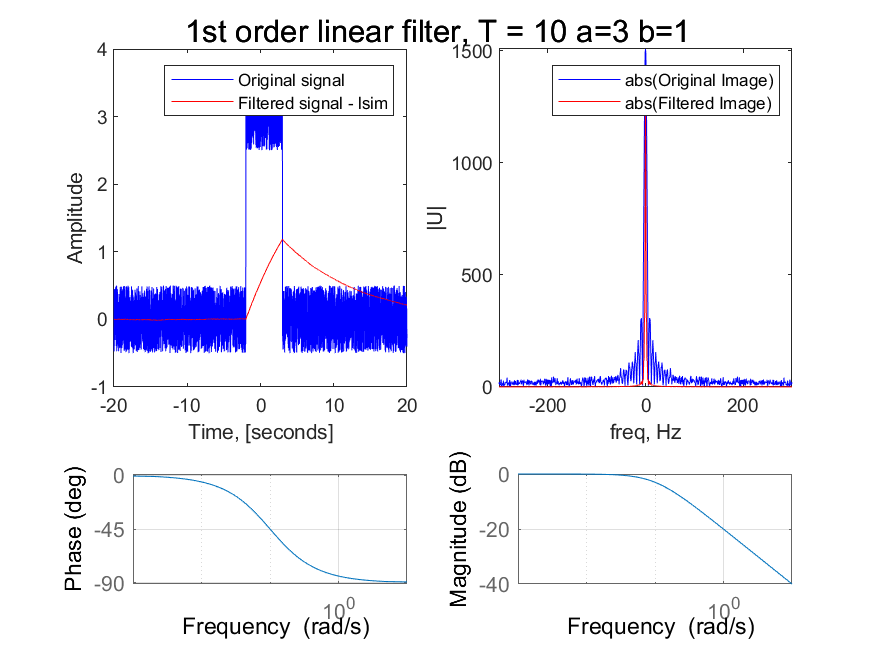
\includegraphics[width=1\textwidth]{test_linear_filter=3_b=1_T=10_00.png }
	\caption{Испытание 4}
\end{figure}

\begin{figure}[ht]
    \centering
    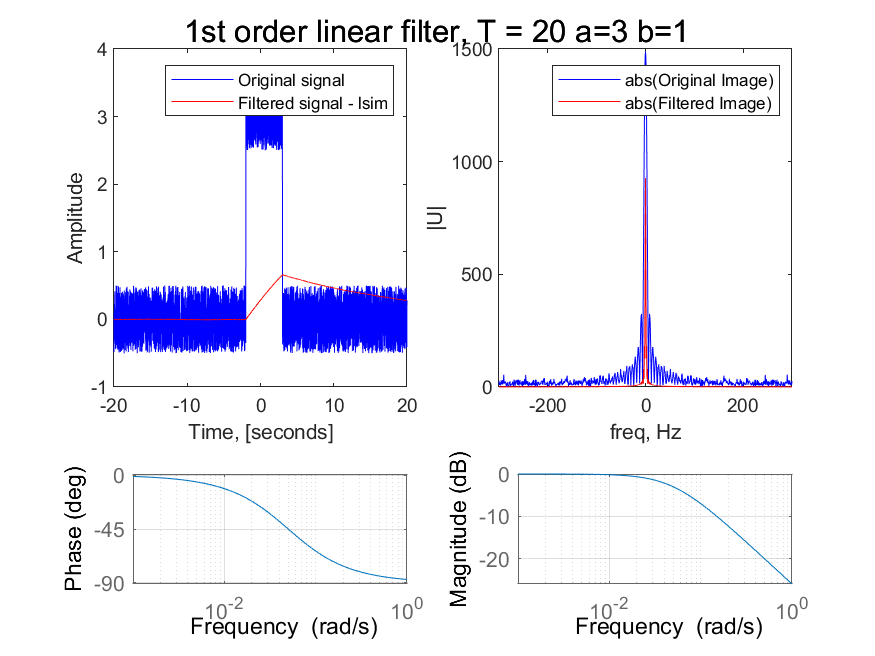
\includegraphics[width=1\textwidth]{test_linear_filter=3_b=1_T=20_00.png}
	\caption{Испытание 5}
\end{figure}
\newpage
\begin{figure}[ht]
    \centering
    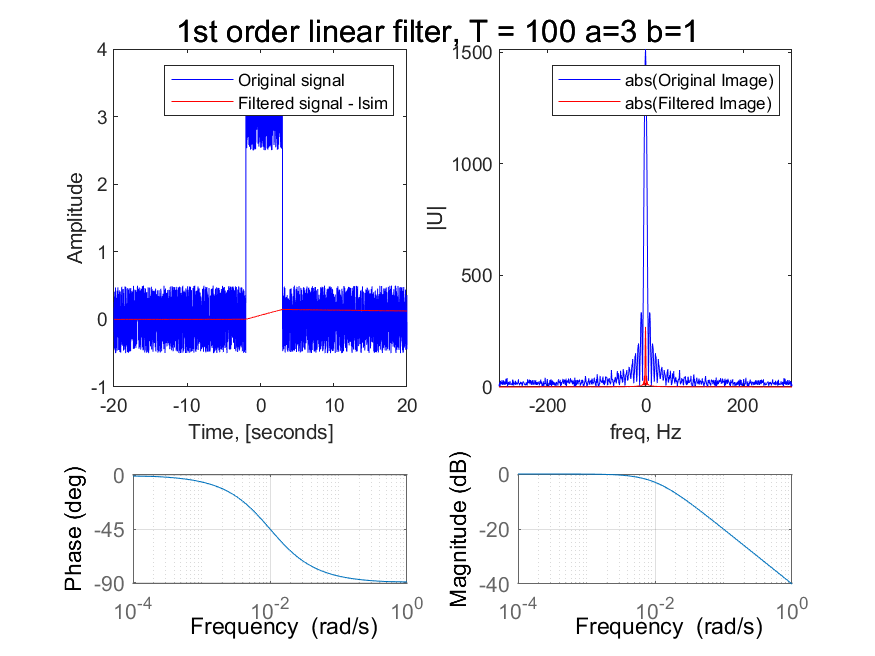
\includegraphics[width=1\textwidth]{test_linear_filter=3_b=1_T=100_00.png}
	\caption{Испытание 6}
\end{figure}

\begin{figure}[ht]
    \centering
    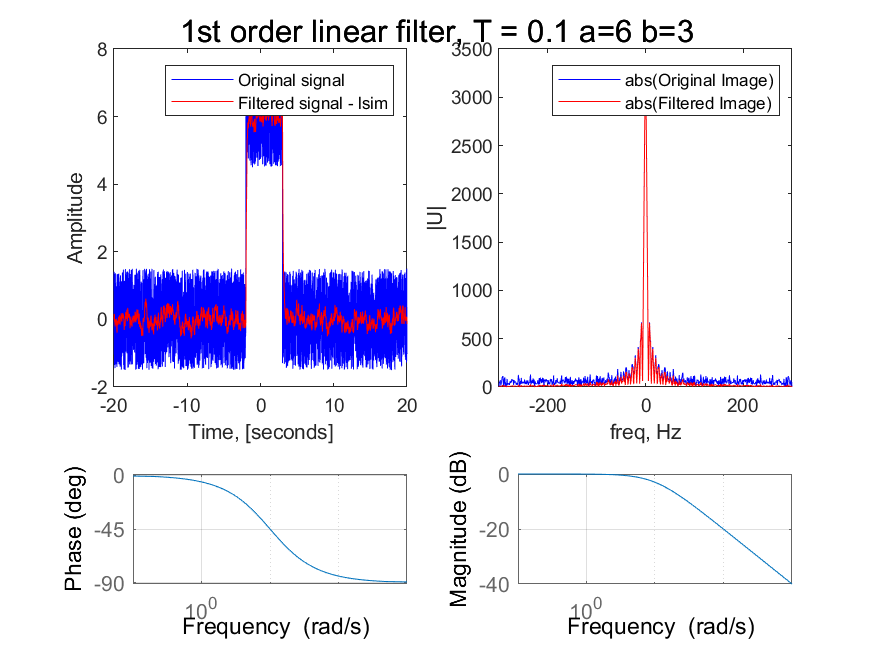
\includegraphics[width=1\textwidth]{test_linear_filter=6_b=3_T=0_10.png}
	\caption{Испытание 7}
\end{figure}
\newpage
\begin{figure}[ht]
    \centering
    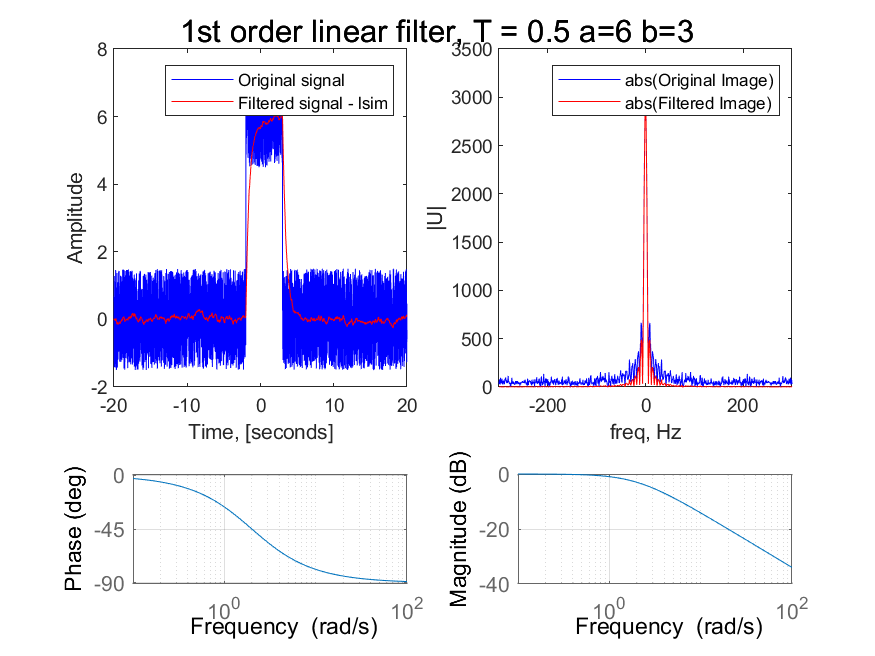
\includegraphics[width=1\textwidth]{test_linear_filter=6_b=3_T=0_50.png }
	\caption{Испытание 8}
\end{figure}

\begin{figure}[ht]
    \centering
    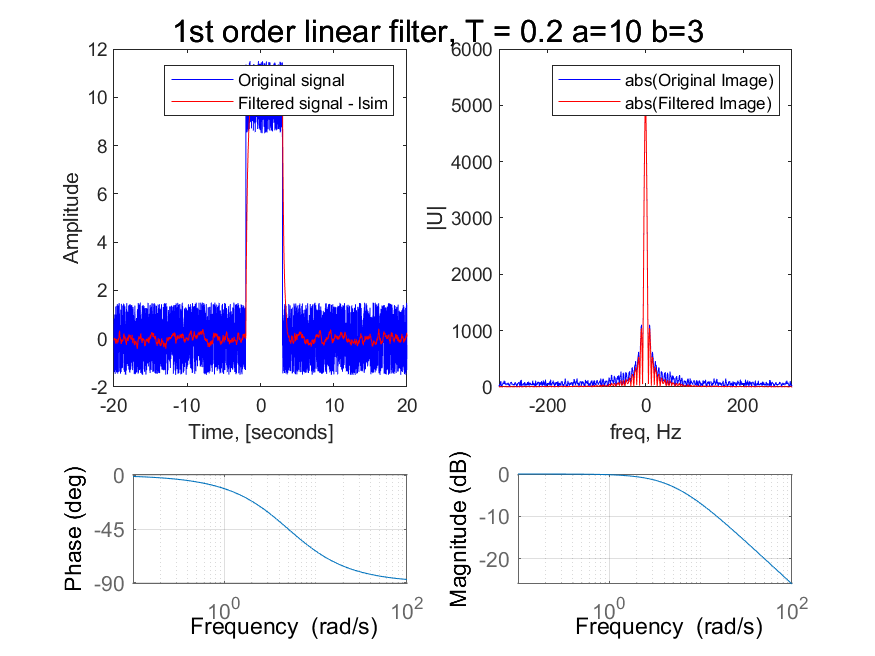
\includegraphics[width=1\textwidth]{test_linear_filter=10_b=3_T=0_20.png}
	\caption{Испытание 9}
\end{figure}


\newpage
\subsection{Выводы}
Давайте исследовать влияние постоянной времени $T$ и значения параметра $a$ на эффективность фильтрации. Возможно это не слишком заметно, но параметр $a$ у нас влияет на добавление белого шума и как бы мы не пытались увеличивать его амплитуду, - фильтр все равно более менее хорошо справлялся с таким шумом.
Но фильтр в первую очередь справлялся из-за хорошо подобранной постоянной времени - больше единицы ставить не было смысла, потому что результат плачевный. Поэтому подбирая на ощупь в пределах $[0 ; 1]$ с шагом $0.1$ можно было достичь приемлимых результатов.




\section{Специальный фильтр}
Выберем только $b=0$, остальные будут как-то заданы. Теперь мы уже имеем дело с двумя компонентами шума - случайным и гармоническим:
$$
\texttt{u = g + b*(rand(size(t))-0.5) + c*sin(d*t);}
$$
\subsection{Испытания}

\begin{figure}[ht]
    \centering
    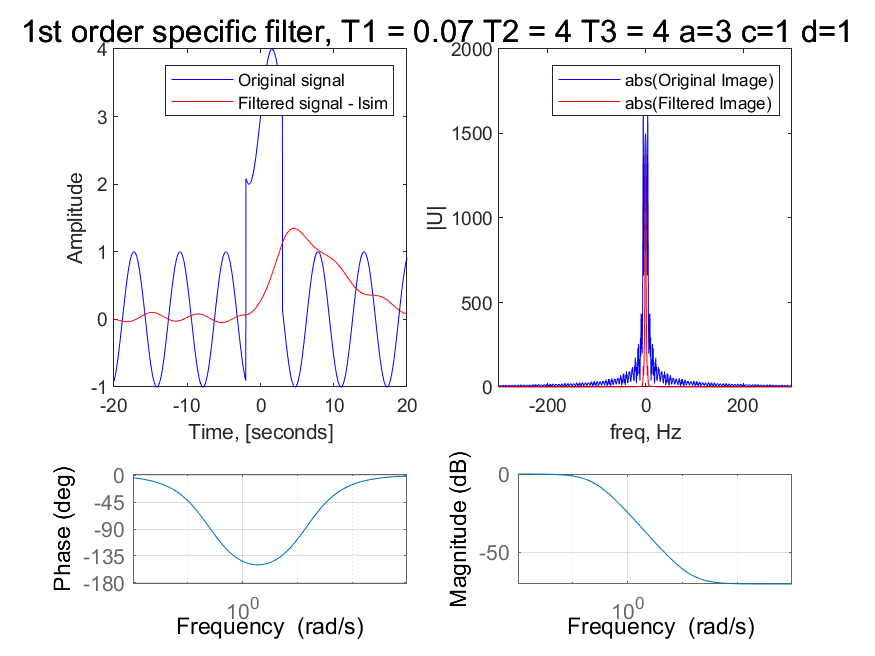
\includegraphics[width=1\textwidth]{test_specific_filter=3_b=0_c=1_d=1_T1=0_07_T2=4_00_T3=4_00.png}
	\caption{Испытание 1}
\end{figure}

\begin{figure}[ht]
    \centering
    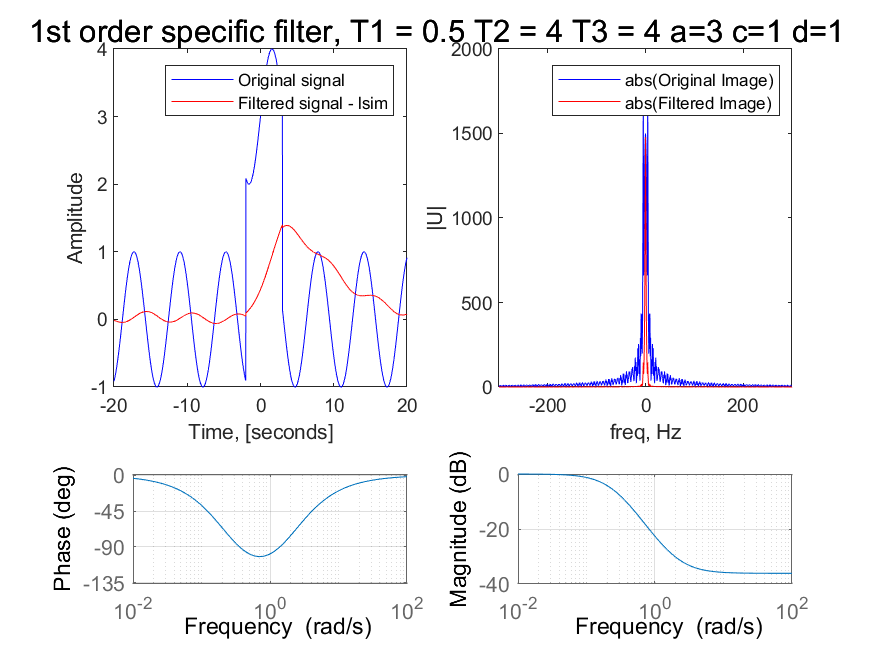
\includegraphics[width=1\textwidth]{test_specific_filter=3_b=0_c=1_d=1_T1=0_50_T2=4_00_T3=4_00.png}
	\caption{Испытание 2}
\end{figure}
\newpage
\begin{figure}[ht]
    \centering
    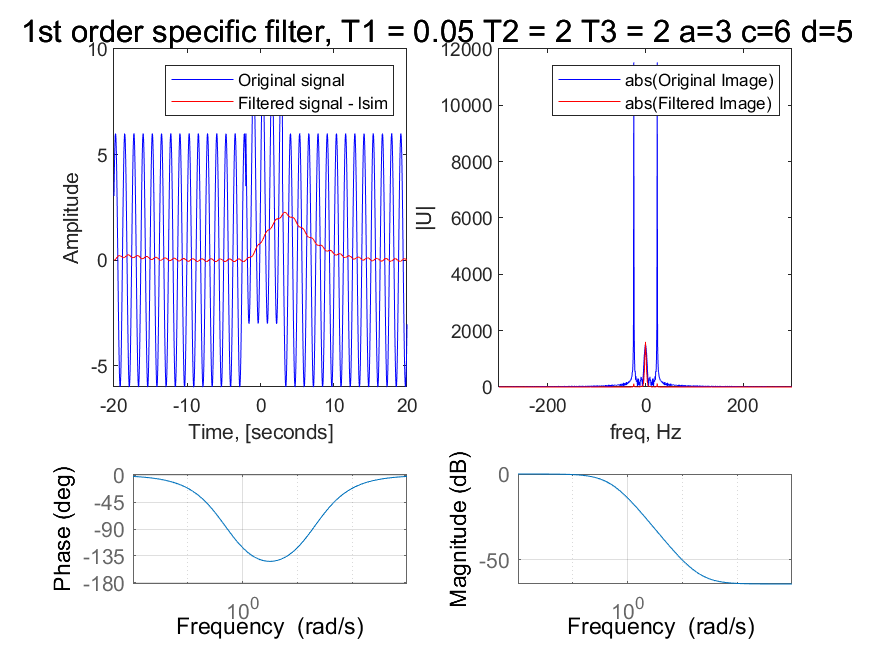
\includegraphics[width=1\textwidth]{test_specific_filter=3_b=0_c=6_d=5_T1=0_05_T2=2_00_T3=2_00.png}
	\caption{Испытание 3}
\end{figure}


\begin{figure}[ht]
    \centering
    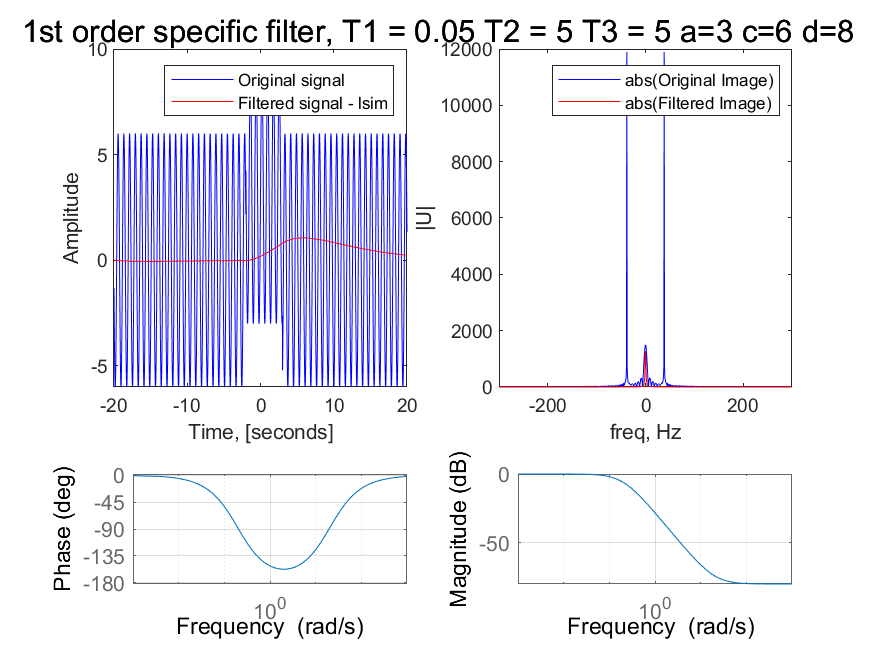
\includegraphics[width=1\textwidth]{test_specific_filter=3_b=0_c=6_d=8_T1=0_05_T2=5_00_T3=5_00.png}
	\caption{Испытание 4}
\end{figure}


\newpage
\newpage
\subsection{Выводы}
Чисто эмпирическим путём удалось выяснить, что похоже, равенство $T_2=T_3$ - даёт очень хорошие результаты. Также при этом $T_1$ должен быть меньше двух остальных коэффциентов, и не сллишком равен им... Поэтому все испытания проводились примерно с таким соотношением.

При большом $c$ мы получаем гармонический шум с большой амплитудой, коэффициенты фильтрации для которого подбираются на глаз куда сложнее, нежели для амплитуд небольших. То же самое было и с параметром $d$, но дело не в этом. 
При небольшом $c$ результат фильтрации выходит самым гладким и точным, 
а при увелечении потери от оригинала как будто значительно увеличиваются.


\endinput 
\chapter{Задание 3. Гладим биржевые данные}
\label{ch:chap3}

\definecolor{codegreen}{rgb}{0,0.6,0}
\definecolor{codegray}{rgb}{0.5,0.5,0.5}
\definecolor{codepurple}{rgb}{0.58,0,0.82}
\definecolor{backcolour}{rgb}{0.95,0.95,0.92}

\lstdefinestyle{mystyle}{
    backgroundcolor=\color{backcolour},   
    commentstyle=\color{codegreen},
    keywordstyle=\color{magenta},
    numberstyle=\tiny\color{codegray},
    stringstyle=\color{codepurple},
    basicstyle=\ttfamily\footnotesize,
    breakatwhitespace=false,         
    breaklines=true,                 
    captionpos=b,                    
    keepspaces=true,                 
    numbers=left,                    
    numbersep=5pt,                  
    showspaces=false,                
    showstringspaces=false,
    showtabs=false,                  
    tabsize=2
}

\lstset{style=mystyle}

Выбираем какую-нибудь котировку ценной бумаги, у меня матлаб ругался на акции РосНефти по неизвестной мне причине, поэтому пришлось брать базовую базу, а именно всеми любимые зелёные бумажки (Сбербанк).
На этом \href{https://drive.google.com/drive/folders/1o8ozGv-bwYWuNpUlfYqM3rDu85QSQ0JW}{сайте} задали временной промежуток в 4 года и скачали \texttt{.csv} файл, с которым будем работать далее.

\section{Сравнительные графики исходного и фильтрованного сигналов}

\begin{figure}[ht]
    \centering
    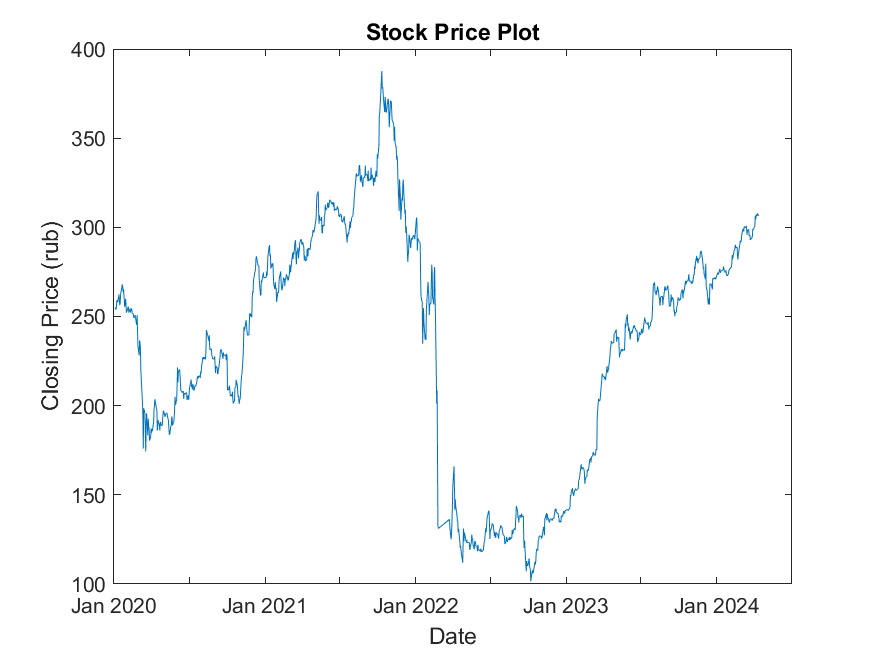
\includegraphics[width=0.8\textwidth]{test_stocks_original_SBER.png}
    \caption{Изначальный график котировки}
\end{figure}

\begin{figure}[ht]
    \centering
    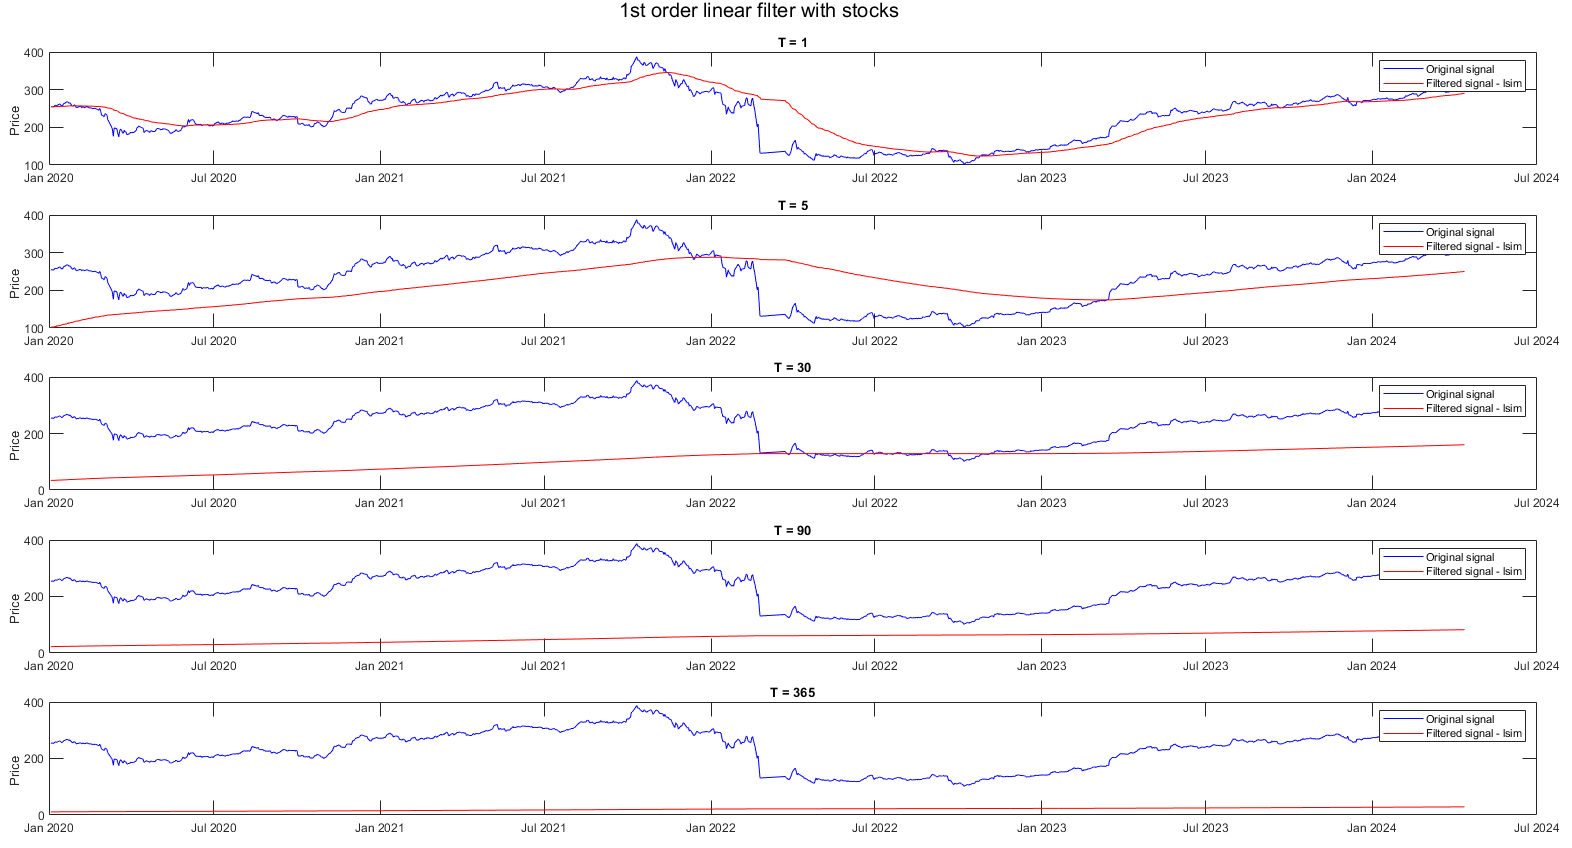
\includegraphics[width=1\textwidth]{untitled.png}
    \caption{Сглаживания по всем T}
\end{figure}


Получается, что каждый из подграфиков ниже нужно читать следующим образом: сначала мы сглаживаем "днями", то есть минимальный единичный отрезок при фильтрации на оси икс - это день, потом неделя, месяц, год. 
Так как данные у меня взяты за 4 года, то при апроксимации по годам итоговый график совсем плывёт и почти ничего не показывает, потому что для него слишком мало данных - всего 4 точки(4 года).

\endinput

% \printbibliography[title=Список использованных источников] % Автособираемый список литературы

\end{document}